% Calibrated merger simulation: mechanics and logit vs. linear demand
% Canonical (LaTeX) version of docs/calibrated_merger_simulation.md
% Student-oriented: every formula is derived step by step.
% Compile from the docs/ directory, twice for cross-references:
%   pdflatex calibrated_merger_simulation.tex
\documentclass[11pt,a4paper]{article}
\usepackage[margin=2.5cm]{geometry}
\usepackage{amsmath,amssymb}
\usepackage{graphicx}
\usepackage{booktabs}
\usepackage[table]{xcolor}
\usepackage{url}
\usepackage{caption}
\usepackage{hyperref}
\hypersetup{colorlinks=true,linkcolor=blue,urlcolor=blue,citecolor=blue}

\title{Calibrated Merger Simulation:\\ Mechanics, and Logit vs.\ Linear Demand\\[4pt]
\large A student-friendly derivation of the method and the code}
\author{merger-sim project}
\date{\today}

\begin{document}
\maketitle

\begin{abstract}
This note explains the calibrated merger simulation implemented in
\path|python/mergersim/|, deriving every formula step by step: the three-step recipe
(calibrate demand from pre-merger shares, prices and margins; impute marginal costs from
the Nash--Bertrand first-order conditions; re-solve the pricing game under the post-merger
ownership matrix), a side-by-side treatment of \emph{logit} and \emph{linear} demand with
full derivations, the diagnostics used in practice (diversion ratios, HHI, upward pricing
pressure, welfare), figures, worked examples, exercises, and pointers to the exact lines
of code implementing each piece. The literature is reviewed in
\path|docs/literature.md| \cite{farrell1990,farrell2010,hlz1994,werden1994,blp1995,nevo2001,peters2006,budzinski2010,nevoWhinston2010}.
\end{abstract}

\section{The three-step recipe}
\label{sec:recipe}

A calibrated merger simulation predicts the effect of a hypothetical horizontal merger
using only \emph{pre-merger} data. The standard recipe \cite{hlz1994,werden1994}:
\begin{enumerate}
\item \textbf{Calibrate demand} for the $J$ products in the market from observed shares
  $s_j$, prices $p_j$ and margins $m_j = p_j - c_j$. Implemented in
  \path|LogitDemand.calibrate| (\path|demand.py:28|) and \path|LinearDemand.calibrate|
  (\path|demand.py:112|), dispatched by \path|Market.calibrated(..., demand_type=...)|
  (\path|market.py:25|). Derivations in Section~\ref{sec:demand}.
\item \textbf{Impute marginal costs} $c_j = p_j - m_j$ from the pre-merger
  Nash--Bertrand first-order conditions (FOCs) --- this is what identifies the price
  coefficient(s) of the demand system. Sections~\ref{sec:demand}--\ref{sec:supply}.
\item \textbf{Re-solve the pricing game} under the post-merger ownership matrix
  $\Omega^{post}$ and compare equilibria: prices, shares, HHI, diversion ratios,
  upward pricing pressure (UPP), profits and consumer surplus. Implemented in
  \path|simulate_merger| (\path|simulation.py:58|); equilibrium solving in
  \path|Market.solve_prices| (\path|market.py:72|). Algorithm in Section~\ref{sec:algorithm}.
\end{enumerate}

A lighter-weight screen that skips step~3 is \textbf{UPP} \cite{farrell2010}, computed
in \path|upward_pricing_pressure| (\path|simulation.py:45|) --- derived in
Section~\ref{sec:diagnostics}.

\section{Setup and notation}
\label{sec:setup}

One market with $J$ differentiated products, market size $M$ (population; per-capita
analysis is $M=1$), and firms $f=1..F$ with ownership matrix
\begin{equation}\label{eq:omega}
\Omega_{ij} = \mathbf{1}\{\text{products } i,j \text{ owned by the same firm}\}\ .
\end{equation}
Code: \path|Market.ownership| (\path|python/mergersim/market.py:48|). Quantities
$q_j = M s_j$. Firms set prices simultaneously (Nash--Bertrand); firm $f$ maximises
\begin{equation}\label{eq:profit}
\pi_f = \sum_{j \in f} (p_j - c_j)\, q_j = M \sum_{j \in f} m_j\, s_j .
\end{equation}

\section{Demand systems: full derivations}
\label{sec:demand}

\subsection{Logit demand --- \texttt{LogitDemand} (\texttt{demand.py:19})}
\label{sec:logit}

\subsubsection*{Step 1: from random utility to shares}
Consumer $h$ gets utility $u_{hj} = \delta_j + \varepsilon_{hj}$ from product $j$ and
$u_{h0} = \varepsilon_{h0}$ from the outside good, with $\varepsilon$ i.i.d.\ type-I
extreme value. The probability of choosing $j$ is the multinomial logit
\begin{equation}\label{eq:logit}
s_j = \Pr(j) = \frac{e^{\delta_j}}{\sum_{k=0}^{J} e^{\delta_k}}
     = \frac{e^{\delta_j}}{1 + \sum_{k=1}^{J} e^{\delta_k}},
\end{equation}
where we normalise $\delta_0 \equiv 0$. Write the linear-in-price mean utility as
\begin{equation}\label{eq:delta}
\delta_j(p) = \beta_j - a\, p_j, \qquad a > 0 .
\end{equation}
Code: \path|LogitDemand.shares| (\path|demand.py:55|) evaluates \eqref{eq:logit}--\eqref{eq:delta}
with \path|delta_j = intercepts_j - a * p_j|.

\subsubsection*{Step 2: inverting the share equation (Berry 1994)}
Divide \eqref{eq:logit} by the outside share $s_0 = 1-\sum_j s_j$:
$$\frac{s_j}{s_0} = e^{\delta_j} \quad\Longrightarrow\quad
\delta_j = \ln s_j - \ln s_0 .$$
So observed shares pin down the \emph{levels} $\delta_j$; the price coefficient $a$
comes from the supply side (Step 5).

\subsubsection*{Step 3: the demand Jacobian and elasticities}
Let $D = 1 + \sum_k e^{\delta_k}$, so $s_j = e^{\delta_j}/D$ and, from
\eqref{eq:delta}, $\partial \delta_k/\partial p_k = -a$ (and $0$ for $k \neq j$ when
differentiating w.r.t.\ $p_j$). Quotient rule:
\begin{align}
\frac{\partial s_j}{\partial p_j}
  &= \frac{e^{\delta_j}(-a)\,D - e^{\delta_j}\big(e^{\delta_j}(-a)\big)}{D^2}
   = -a\, s_j + a\, s_j^2 = -a\, s_j (1 - s_j), \label{eq:dlogitown}\\
\frac{\partial s_j}{\partial p_k} \;(k \neq j)
  &= \frac{0 - e^{\delta_j}\big(e^{\delta_k}(-a)\big)}{D^2}
   = a\, s_j s_k . \label{eq:dlogitcross}
\end{align}
Hence elasticities $\varepsilon_{ji} = (p_i/s_j)\,\partial s_j/\partial p_i$:
$$\varepsilon_{jj} = -a\, p_j (1-s_j) < 0, \qquad
\varepsilon_{jk} = a\, p_k s_j > 0 \;(j \neq k).$$
Code: \path|LogitDemand.jacobian| (\path|demand.py:66|) returns $A_{ji} = \partial
s_j/\partial p_i = a\, s_j (s_i - \mathbf{1}[j=i])$, which is exactly
\eqref{eq:dlogitown}--\eqref{eq:dlogitcross}; \path|elasticities| (\path|demand.py:71|)
scales by $p_i/s_j$.

\subsubsection*{Step 4: diversion ratios}
The diversion ratio from $i$ to $j$ is the share of $i$'s lost sales that go to $j$:
\begin{equation}\label{eq:divdef}
D_{ij} \equiv -\frac{\partial s_j/\partial p_i}{\partial s_i/\partial p_i} .
\end{equation}
Using \eqref{eq:dlogitown}--\eqref{eq:dlogitcross} ($i \neq j$):
$$D_{ij} = -\frac{a\, s_i s_j}{-a\, s_i (1-s_i)} = \frac{s_j}{1-s_i} .$$
Code: \path|LogitDemand.diversion_ratios| (\path|demand.py:77|). Note $D_{ij}$ varies with
prices through $s$ (Fig.~\ref{fig:div}), and $\sum_{j \neq i} D_{ij} = (1 - s_0 - s_i)/(1-s_i) < 1$:
not all diverted sales stay inside the market --- the outside good absorbs the rest.

\subsubsection*{Step 5: the supply FOC identifies $a$ (calibration)}
A single-product firm $j$ maximises $\pi_j = M (p_j - c_j) s_j(p)$:
$$0 = \frac{\partial \pi_j}{\partial p_j}
   = M\Big[ s_j + (p_j - c_j)\, \frac{\partial s_j}{\partial p_j} \Big]
   \overset{\eqref{eq:dlogitown}}{=} M\Big[ s_j - a\,(p_j-c_j)\, s_j (1-s_j) \Big] .$$
Divide by $M s_j > 0$:
\begin{equation}\label{eq:logitfoc}
(p_j - c_j)\, a\, (1 - s_j) = 1
\quad\Longrightarrow\quad
a = \frac{1}{(p_j - c_j)(1 - s_j)} .
\end{equation}
In the model this is the same $a$ for every product; in data the per-product values
differ (especially with multi-product firms), so the code averages them:
$a = \operatorname{mean}_j 1/[(p_j-c_j)(1-s_j)]$, then $\beta_j = \delta_j + a\, p_j$
(Step 2). Code: \path|LogitDemand.calibrate| (\path|demand.py:28|). If only a Lerner
margin $L$ is known, use $p_j - c_j = L\, p_j$.

\subsubsection*{Step 6: consumer surplus}
With quasi-linear utility, the expected maximum utility (Gumbel) is, up to an additive
constant,
$$V(p) = \frac{1}{a} \ln\!\Big(1 + \sum_j e^{\delta_j(p)}\Big) .$$
Check Roy's identity: $\partial V/\partial p_j = \frac{1}{a}\cdot\frac{-a\, e^{\delta_j}}{D}
= -s_j$, so $s_j = -\partial V/\partial p_j$ as it must be. For quasi-linear preferences
the change in consumer surplus from $p^0$ to $p^1$ is
\begin{equation}\label{eq:logitCS}
\Delta CS = M\big[ V(p^1) - V(p^0) \big]
          = \frac{M}{a}\Big[ \ln\big(1+\textstyle\sum_j e^{\delta_j(p^1)}\big)
                        - \ln\big(1+\textstyle\sum_j e^{\delta_j(p^0)}\big) \Big] .
\end{equation}
Code: \path|LogitDemand.consumer_surplus| (\path|demand.py:84|) returns the per-capita
$V(p)$; \path|_snapshot| (\path|simulation.py:31|) multiplies by $M$.

\subsection{Linear demand --- \texttt{LinearDemand} (\texttt{demand.py:92})}
\label{sec:linear}

Per-capita linear demand over the inside goods only (no outside good):
\begin{equation}\label{eq:linear}
s(p) = a - B\, p, \qquad q = M\, s, \qquad B_{ji} = -\frac{\partial s_j}{\partial p_i},
\end{equation}
$B_{jj} > 0$, $B_{ij} \le 0$ for substitutes. Code: \path|shares| (\path|demand.py:132|),
\path|jacobian| returns the constant $-B$ (\path|demand.py:141|).

\subsubsection*{Step 1: the utility behind it}
Take quadratic utility $U(s) = \alpha^{\top} s - \tfrac12 s^{\top} B^{-1} s$. The
consumer maximises $U(s) - p^{\top} s$: FOC $\alpha - B^{-1} s - p = 0$, so
$s = B(\alpha - p) = B\alpha - B p$, i.e.\ \eqref{eq:linear} with $a = B\alpha$, or
$\alpha = B^{-1} a$.

\subsubsection*{Step 2: calibration --- own slopes from margins, cross slopes need diversion}
Single-product firm $j$: $q_j = M s_j$, $\partial q_j/\partial p_j = -M B_{jj}$. FOC:
$$0 = q_j + (p_j - c_j)\frac{\partial q_j}{\partial p_j}
   = M s_j - M B_{jj} (p_j - c_j)
\;\Longrightarrow\;
B_{jj} = \frac{s_j}{m_j} \quad \text{(per capita)} .$$
This identifies only the diagonal of $B$. The off-diagonal comes from diversion ratios
(\eqref{eq:divdef}): with \eqref{eq:linear},
$$D_{ij} = -\frac{\partial s_j/\partial p_i}{\partial s_i/\partial p_i}
        = -\frac{-B_{ji}}{-B_{ii}} = -\frac{B_{ji}}{B_{ii}}
\;\Longrightarrow\;
B_{ji} = -D_{ij}\, B_{ii} .$$
Code: \path|LinearDemand.calibrate| (\path|demand.py:112|) sets $B_{jj}=s_j/m_j$ and
$B_{ij}=-D_{ij}B_{jj}$; by default it proxies $D_{ij}=s_j/(1-s_i)$ (the logit formula, as
in \cite{farrell2010}'s $REC\cdot s_j/(1-s_i)$), or you pass \path|diversion=|. Then
$a = s + B p$. \textbf{This is the key identification difference vs.\ logit}: one market's
$(s,p,m)$ gives one scalar under logit, but only the own slopes under linear demand.

\subsubsection*{Step 3: closed-form Nash--Bertrand equilibrium}
The general FOC (derived in Section~\ref{sec:supply}) is
$r = s - B^{\top}(\Omega\, m) = 0$ for linear demand (since $\partial s_k/\partial p_i =
-B_{ki}$). Substitute $s = a - B p$ and $m = p - c$:
$$a - B p = B^{\top}\Omega (p - c)
\;\Longrightarrow\;
(B + B^{\top}\Omega)\, p = a + B^{\top}\Omega\, c ,$$
\begin{equation}\label{eq:closedform}
p^{*} = (B + B^{\top}\Omega)^{-1}\,(a + B^{\top}\Omega\, c) .
\end{equation}
Code: \path|LinearDemand.closed_form_prices| (\path|demand.py:165|); used by
\path|Market.solve_prices| (\path|market.py:72|).

\subsubsection*{Step 4: consumer surplus}
$CS(p) = U(s(p)) - p^{\top} s(p)$ with $U$ from Step 1 and $\alpha = B^{-1}a$:
\begin{equation}\label{eq:linearCS}
CS(p) = \alpha^{\top} s - \tfrac12 s^{\top} B^{-1} s - p^{\top} s,
\qquad s = a - Bp .
\end{equation}
Code: \path|LinearDemand.consumer_surplus| (\path|demand.py:157|).

\subsubsection*{Caveats}
Shares can go \emph{negative} at high prices (Fig.~\ref{fig:demand}); inside shares sum
to one (no outside good --- the cereal data's inside shares sum to $\approx 0.70$);
diversion ratios are \emph{constant} in prices (Fig.~\ref{fig:div}); niche products can
get implausible corner prices after a merger (Fig.~\ref{fig:cereal}).

\subsection{Logit vs.\ linear at a glance}

\begin{table}[h]
\centering
\caption{Logit vs.\ linear demand in the calibrated simulation}
\label{tab:compare}
\begin{tabular}{@{}lll@{}}
\toprule
property & logit & linear \\
\midrule
shares & bounded in $(0,1)$, outside good $s_0>0$ & can go negative; $\sum_j s_j = 1$ \\
price coef(s) identified from $(s,p,m)$ & one scalar $a$, Eq.~\eqref{eq:logitfoc} & own slopes $B_{jj}=s_j/m_j$ only; cross slopes need $D$ \\
diversion $D_{ij}$ & $s_j/(1-s_i)$, varies with prices & $-B_{ij}/B_{jj}$, constant \\
post-merger equilibrium & numerical (fixed point $+$ root finding) & closed form, Eq.~\eqref{eq:closedform} \\
consumer surplus & closed form, Eq.~\eqref{eq:logitCS} & quadratic form, Eq.~\eqref{eq:linearCS} \\
code & \path|demand.py:19--90| & \path|demand.py:92--168| \\
\bottomrule
\end{tabular}
\end{table}

\begin{figure}[h]
\centering
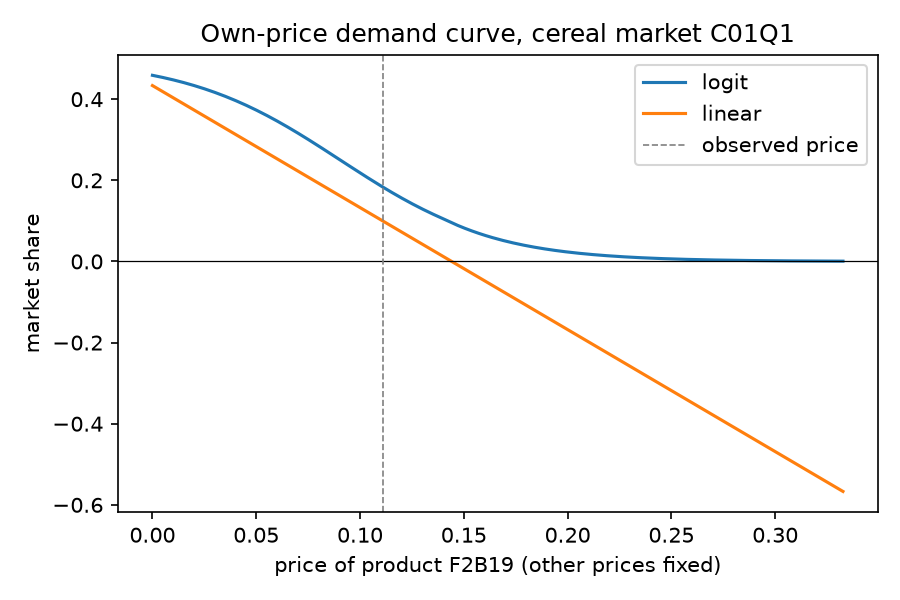
\includegraphics[width=0.75\textwidth]{figures/fig1_demand_forms.png}
\caption{Own-price demand curve for product F2B19 in cereal market C01Q1 (calibrated at
the observed price, dashed line), other prices fixed. The logit curve stays in $(0,1)$
and flattens as the outside good absorbs demand; the linear curve is a straight line
that crosses zero. Generated by \texttt{python/examples/make\_figures.py:20}.}
\label{fig:demand}
\end{figure}

\begin{figure}[h]
\centering
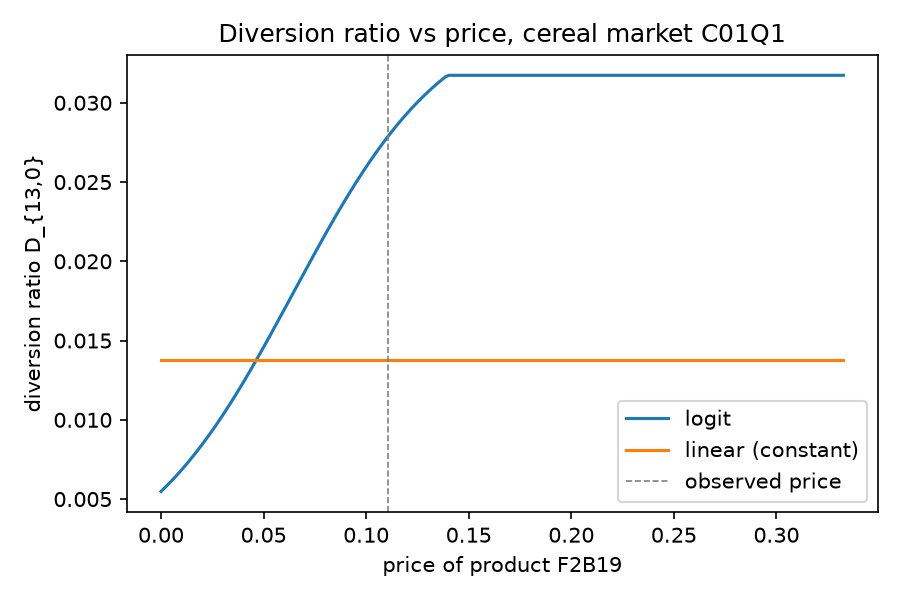
\includegraphics[width=0.75\textwidth]{figures/fig2_diversion_forms.png}
\caption{Diversion ratio $D_{ij}$ as the price of product $i$ varies: logit's
share-proportional diversion falls as $p_i$ rises; linear's is constant.}
\label{fig:div}
\end{figure}

\section{Supply side: FOCs, ownership matrix, equilibrium solvers}
\label{sec:supply}

\subsection{The multi-product FOC with the ownership matrix}
Firm $f$ maximises \eqref{eq:profit}. For product $i \in f$:
$$\frac{\partial \pi_f}{\partial p_i}
 = M\Big[ s_i + \sum_{j \in f} (p_j - c_j)\, \frac{\partial s_j}{\partial p_i} \Big] = 0 .$$
Using $\Omega$ (\eqref{eq:omega}), $j \in f \iff \Omega_{ij}=1$, and $A_{ji} =
\partial s_j/\partial p_i$:
\begin{equation}\label{eq:foc}
r_i(p) = s_i + \sum_{k} \Omega_{ik}\, m_k\, A_{ki} = 0
\qquad \text{for all } i .
\end{equation}
Code: \path|Market.foc| (\path|python/mergersim/market.py:63|) --- generic over the demand
class via \path|demand.shares| and \path|demand.jacobian|.

\subsection{Solving for equilibrium prices}
\path|Market.solve_prices| (\path|market.py:72|) collects candidates and returns the one
with the smallest FOC residual:
\begin{itemize}
\item \textbf{linear demand}: closed form \eqref{eq:closedform} (\path|demand.py:165|);
\item \textbf{logit demand}: markup fixed-point iteration \cite{morrow2011}. Derivation:
  insert the logit Jacobian into \eqref{eq:foc}:
  $$r_i = s_i + \sum_{k \in f} m_k\, a\, s_k (s_i - \mathbf{1}[k=i]) = 0
       = s_i + a\, s_i \Big[ m_i (1-s_i) - \textstyle\sum_{k \in f,\, k \neq i} m_k s_k \Big] .$$
  Divide by $a s_i$ and solve for $m_i$:
  \begin{equation}\label{eq:fp}
  m_i = \frac{1/a + \sum_{k \in f,\, k \neq i} m_k s_k}{1 - s_i},
  \qquad p_i = c_i + m_i .
  \end{equation}
  Iterate from observed prices. Code: \path|Market._fixed_point| (\path|market.py:96|).
\item \textbf{both}: \texttt{scipy.optimize.root} on the FOCs as fallback/refinement.
\end{itemize}

Pre-merger, observed prices should satisfy the FOCs (this is what identifies demand/costs).
Tests: \path|test_premerger_foc_holds| (\path|python/tests/test_mergersim.py:39|);
calibration recovery: \path|test_calibration_recovers_a| and \path|test_calibration_recovers_B|
(\path|python/tests/test_linear.py:12|).

\section{The merger simulation algorithm --- \texttt{simulate\_merger} (\texttt{simulation.py:58})}
\label{sec:algorithm}

Given a calibrated \path|Market| and merging firms $M_{set}$:
\begin{enumerate}
\item \textbf{New ownership}: all products of firms in $M_{set}$ get one firm id
  $\to \Omega^{post}$ (\path|simulation.py| lines 64--66).
\item \textbf{Efficiencies}: \texttt{efficiency} $E$ is a proportional marginal-cost
  saving on the merging firms' products: $c_j^{post} = (1-E)c_j$ (lines 67--69).
\item \textbf{Re-solve equilibrium}: $p^{post}$ = \path|Market.solve_prices| under
  $\Omega^{post}$, starting from observed prices (line 71).
\item \textbf{Compare}: \path|_snapshot| (\path|simulation.py:31|) computes pre and post:
  prices, shares, quantities, margins, per-firm profits (\path|Market.profits|,
  \path|market.py:110|), HHI on inside shares renormalised to sum to 1
  (\path|Market.hhi|, \path|market.py:58|), consumer surplus $M \cdot CS(p)$.
\item \textbf{Diagnostics}: UPP (Section~\ref{sec:diagnostics}), diversion matrix,
  per-product table via \path|report| (\path|simulation.py:86|).
\end{enumerate}

Usage (\path|python/examples/run_cereal_merger.py:13|):
\begin{verbatim}
m = nevo_market("C01Q1", lerner=0.3, demand_type="logit")  # or "linear"
res = simulate_merger(m, merging_firms=[1, 2], efficiency=0.05)
table, summary = report(res)  # per-product price/share changes + UPP; HHI/CS/profit
\end{verbatim}

\section{Diagnostics: HHI, diversion, welfare, and the UPP derivation}
\label{sec:diagnostics}

\textbf{HHI}: \path|Market.hhi| (\path|market.py:58|),
$10000 \sum_f (s_f / \sum_g s_g)^2$. \textbf{Diversion}: \path|demand.diversion_ratios|
(\path|demand.py:77| / \path|:151|). \textbf{Welfare}: consumer surplus $+$ total profit,
pre vs.\ post (\path|report|).

\subsection{Deriving UPP (Farrell--Shapiro 2010), two-product case}
Two single-product firms 1 and 2 merge. Pre-merger FOC for product $i$ (from
\eqref{eq:logitfoc}): $1/a = m_i (1 - s_i)$. Post-merger, the merged firm internalises
product $j$'s sales when pricing $i$; the FOC is (\eqref{eq:foc} with $\Omega_{ij}=1$):
$$s_i - a\, m_i'\, s_i (1-s_i) + a\, m_j\, s_i s_j = 0 ,$$
where $m_i' = p_i - c_i'$ and $c_i' = (1-E_i) c_i$. Divide by $a s_i$:
$$\frac{1}{a} - m_i'(1-s_i) + m_j s_j = 0 .$$
Linearise around pre-merger prices: $m_i' \approx m_i + \Delta p_i + E_i c_i$, and use the
pre-merger condition $1/a = m_i (1-s_i)$:
$$-(\Delta p_i + E_i c_i)(1 - s_i) + m_j s_j = 0
\;\Longrightarrow\;
\Delta p_i = \frac{m_j s_j}{1 - s_i} - E_i c_i
          = D_{ij}\, m_j - E_i c_i ,$$
because $D_{ij} = s_j/(1-s_i)$ (\eqref{eq:divdef} + logit Jacobian). So
\begin{equation}\label{eq:upp}
\boxed{\; UPP_i = D_{ij}\,(p_j - c_j) - E_i\, c_i \;}
\end{equation}
is the first-order prediction of $\Delta p_i$: prices rise iff $UPP_i > 0$ (in the
multi-product case, $UPP_i = \sum_{j \in M_{set},\, j \neq i} D_{ij} m_j - E_i c_i$).
Code: \path|upward_pricing_pressure| (\path|simulation.py:45|) --- exactly this formula.

\textbf{Worked example.} $s_i = s_j = 0.2$, $p_i = p_j = \$1$, $c_i = c_j = \$0.70$, no
efficiencies. Then $D_{ij} = 0.2/0.8 = 0.25$, margin $m_j = 0.30$, so
$UPP_i = 0.25 \times 0.30 = 0.075$: the local approximation predicts $\Delta p_i \approx
+\$0.075$ (+7.5\%). The full simulation differs because demand re-equilibrates
(pass-through), but the \emph{sign} is robust \cite{farrell2010}:

\begin{figure}[h]
\centering
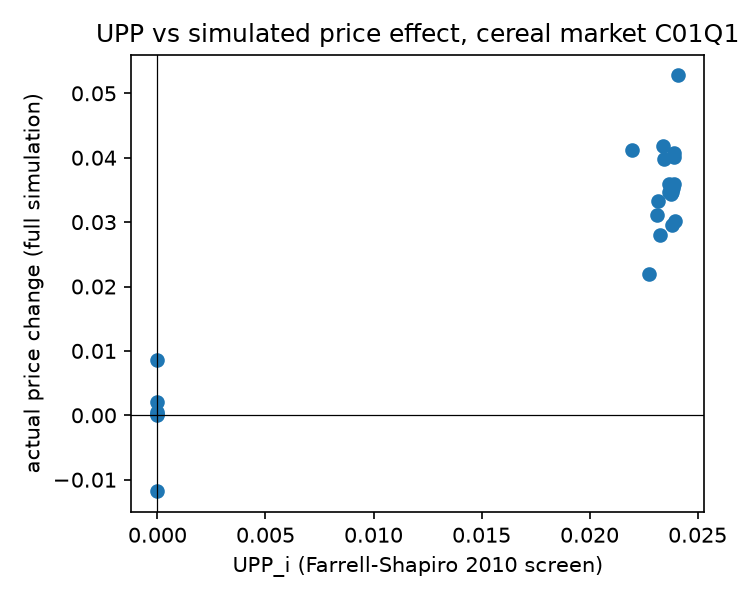
\includegraphics[width=0.6\textwidth]{figures/fig4_upp_vs_dp.png}
\caption{UPP$_i$ vs.\ the full-simulation price change $\Delta p_i$ (logit, cereal
C01Q1, firms 1+2): positive UPP $\iff$ positive $\Delta p$, but magnitudes differ.}
\label{fig:upp}
\end{figure}

\section{Numerical illustration: same merger, two demand forms}
\label{sec:numerics}

Cereal market C01Q1 (24 products, 5 firms), constant Lerner margin 0.3 (no cost column in
the data), merger of firms 1 and 2, no efficiencies. Run:
\path|PYTHONPATH=python python python/examples/run_logit_vs_linear.py|
(\path|examples/run_logit_vs_linear.py:14|).

\begin{table}[h]
\centering
\caption{Merger of firms 1 and 2, cereal market C01Q1: logit vs.\ linear demand}
\label{tab:cereal}
\begin{tabular}{@{}lrr@{}}
\toprule
 & logit & linear \\
\midrule
mean $\Delta p$ of merging products & $+29.6\%$ (max $+73.2\%$) & $+176.9\%$ (max $+525.5\%$) \\
min post-merger share & $+0.0027$ (valid) & $-0.59$ (invalid --- linear pathology) \\
HHI & $3593 \to 4134$ & $3593 \to 2890$ (meaningless: negative shares) \\
consumer surplus & $0.0221 \to 0.0127$ & $0.0227 \to 0.0143$ \\
total profit & $0.0312 \to 0.0515$ & $0.0170 \to 0.2497$ \\
max UPP & $0.0241$ & $0.0130$ \\
\bottomrule
\end{tabular}
\end{table}

For a smaller merger (firms 1+3) where linear shares stay positive, the models agree more
closely: logit $+13.3\%$ vs.\ linear $+18.0\%$ mean price change. Takeaways: both predict
the same \emph{sign} (prices rise, CS falls, profits rise --- the no-synergy result of
\cite{farrell1990}), but \textbf{magnitudes are sensitive to the demand form}
\cite{crooke1999}, and linear demand can produce invalid (negative) shares and implausible
corner prices for niche products --- why logit (or richer systems) dominates agency
practice.

\begin{figure}[h]
\centering
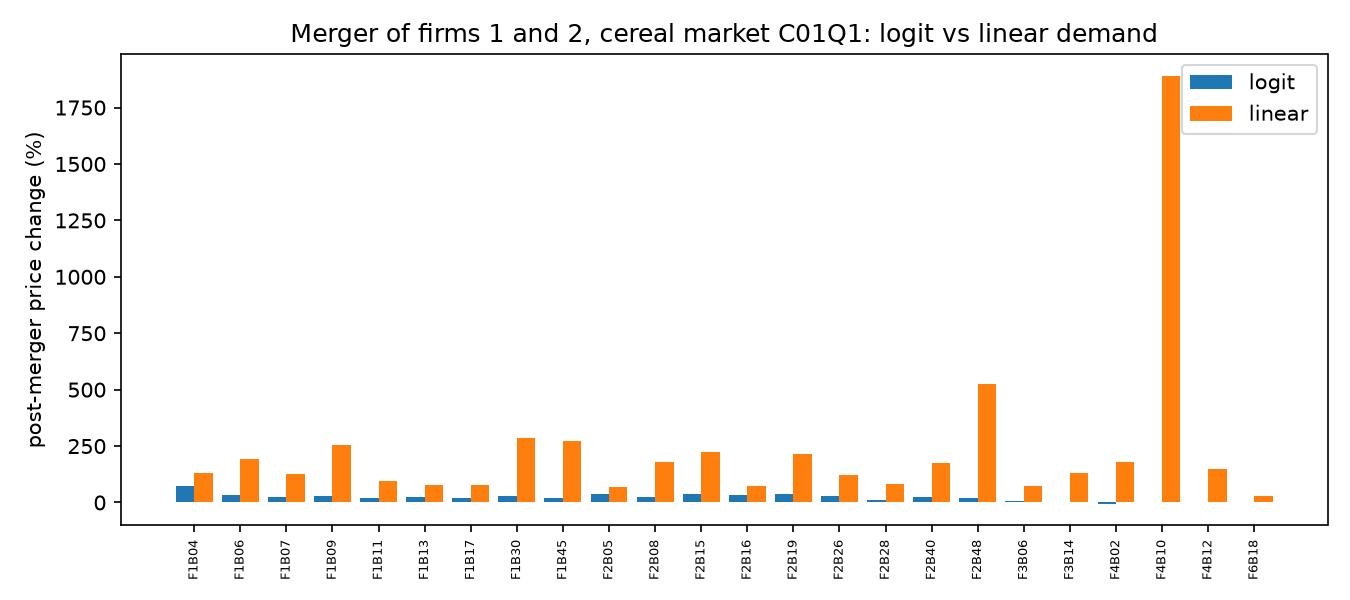
\includegraphics[width=\textwidth]{figures/fig3_cereal_logit_vs_linear.png}
\caption{Per-product post-merger price change, merger of firms 1+2 in cereal market
C01Q1, logit vs.\ linear. Generated by \texttt{python/examples/make\_figures.py:20}.}
\label{fig:cereal}
\end{figure}

\section{Code map}
\label{sec:codemap}

\begin{table}[h]
\centering
\caption{Code map: file $\to$ symbol (line) $\to$ what it does}
\label{tab:codemap}
\begin{tabular}{@{}lll@{}}
\toprule
file & symbol & line \\
\midrule
\path|python/mergersim/demand.py| & \path|LogitDemand| & 19 \\
 & \quad calibration & 28 \\
\path|python/mergersim/demand.py| & \path|LinearDemand| & 92 \\
 & \quad calibration & 112 \\
 & \quad closed-form prices & 165 \\
\path|python/mergersim/market.py| & \path|Market.calibrated| & 25 \\
 & \path|Market.foc| / \path|solve_prices| / \path|_fixed_point| & 63 / 72 / 96 \\
 & \path|Market.hhi|, \path|ownership|, \path|profits|, \path|equilibrium| & 58, 48, 110, 119 \\
\path|python/mergersim/simulation.py| & \path|simulate_merger| & 58 \\
 & \path|upward_pricing_pressure| & 45 \\
 & \path|report| & 86 \\
\path|python/mergersim/data.py| & \path|nevo_market|, \path|synthetic_market|, \path|synthetic_linear_market| & 27, 51, 81 \\
\path|python/examples/| & \path|run_cereal_merger.py|, \path|run_logit_vs_linear.py|, \path|run_synthetic.py|, \path|make_figures.py| & 13, 14, 13, 20 \\
\path|python/tests/| & \path|test_mergersim.py|, \path|test_linear.py| & --- \\
\bottomrule
\end{tabular}
\end{table}

The 19 tests cover: calibration recovery of the true demand parameters, FOC validity pre-
and post-merger, merger price/CS/HHI/UPP properties, and demand-form differences.

\section{Exercises}
\label{sec:exercises}

\begin{enumerate}
\item Redo Step 3 of Section~\ref{sec:logit} (the quotient rule) and verify
  $\sum_j \partial s_j/\partial p_j = -a\, s_j$... check instead that
  $\sum_{j=1}^J \partial s_j/\partial p_i = a s_i (1 - \sum_j s_j)$ --- i.e.\ the outside
  share absorbs the rest. What does this imply for $\sum_{j \neq i} D_{ij}$?
\item Run \path|run_synthetic.py|. Why is the calibrated $a$ exactly the true $a$
  (hint: the synthetic prices are the exact pre-merger equilibrium and firms are
  single-product, so \eqref{eq:logitfoc} holds product by product)?
\item Worked-example check: with $s_i=s_j=0.2$, $p=\$1$, $c=\$0.70$, verify
  $UPP = 0.075$ by hand (Eq.~\eqref{eq:upp}), then compare with
  \path|upward_pricing_pressure| on a synthetic market.
\item Derive the closed-form equilibrium \eqref{eq:closedform} from \eqref{eq:foc} for
  linear demand (Section~\ref{sec:linear}, Step 3) --- write out the matrix algebra.
\item Show that the logit fixed point \eqref{eq:fp} is exactly the FOC \eqref{eq:foc}
  solved for $m_i$ (Section~\ref{sec:supply}). Why is it a contraction for logit demand?
\item Using the calibrated cereal market, find a price $p_k$ at which the \emph{linear}
  share of product $k$ goes negative while the \emph{logit} share stays positive (see
  \path|test_linear_share_unbounded_logit_bounded|). What does this imply for HHI and
  welfare under linear demand after a large merger?
\end{enumerate}

\section{Limitations and natural extensions}
\label{sec:limits}

Background and validation of the method: demand estimation
\cite{berry1994,nevo2000guide,nevo2001,ivaldi2005}; cereal merger applications
\cite{nevo2000}; merger efficiencies and simplified calibration
\cite{froeb2005,epstein2001}; applications and back-tests
\cite{peters2006,bjornerstedt2016,miller2017,gnt2015,nocke2018,doraszelski2008}.

\begin{itemize}
\item \textbf{Richer demand}: nested logit, random-coefficients logit
  \cite{blp1995,nevo2001} --- estimation via PyBLP (\texttt{pyblp}), then feed estimated
  parameters into the same \path|Market| / \path|simulate_merger| machinery; AIDS
  \cite{hlz1994} as an alternative.
\item \textbf{Multi-market}: loop \path|nevo_market| over all 94 cereal markets and
  average effects.
\item \textbf{Efficiencies} (\texttt{efficiency=} in \path|simulate_merger|), product
  repositioning, entry, and dynamic effects \cite{doraszelski2008} are not modelled.
\item \textbf{Bargained prices} (hospitals, \cite{gnt2015}) need a different conduct
  assumption than Nash--Bertrand.
\item \textbf{Linear demand caveats} (Section~\ref{sec:linear}): use it for small price
  changes / teaching; prefer logit$+$ when an outside good matters or price changes are
  large.
\end{itemize}

\begin{thebibliography}{99}

\bibitem{farrell1990}
J.~Farrell and C.~Shapiro, ``Horizontal Mergers: An Equilibrium Analysis,''
\emph{American Economic Review} 80(1):107--126, 1990.

\bibitem{farrell2010}
J.~Farrell and C.~Shapiro, ``Antitrust Evaluation of Horizontal Mergers: An Economic
Alternative to Market Definition,'' \emph{B.E. Journal of Theoretical Economics}
10(1), Article 9, 2010. Open access: \url{https://faculty.haas.berkeley.edu/shapiro/alternative.pdf}

\bibitem{hlz1994}
J.~Hausman, G.~Leonard and J.\,D.~Zona, ``Competitive Analysis with Differentiated
Products,'' \emph{Annales d'\'Economie et de Statistique} 34:159--180, 1994.

\bibitem{werden1994}
G.~Werden and L.~Froeb, ``The Effects of Mergers in Differentiated Products Industries:
Logit Demand and Merger Policy,'' \emph{Journal of Law, Economics, and Organization}
10(2):407--426, 1994.

\bibitem{crooke1999}
P.~Crooke, L.~Froeb, S.~Tschantz and G.~Werden, ``Effects of Assumed Demand Form on
Simulated Post-Merger Equilibria,'' \emph{Review of Industrial Organization}
15:205--220, 1999.

\bibitem{froeb2005}
L.~Froeb, S.~Tschantz and G.~Werden, ``The Effects of Merger Efficiencies on Consumers of
Differentiated Products,'' \emph{European Competition Journal} 4(2):245--262, 2005.

\bibitem{epstein2001}
R.~Epstein and D.~Rubinfeld, ``Merger Simulation: A Simplified Approach with New
Applications,'' UC Berkeley working paper, 2001.

\bibitem{berry1994}
S.~Berry, ``Estimating Discrete-Choice Models of Product Differentiation,''
\emph{RAND Journal of Economics} 25(2):242--262, 1994.

\bibitem{blp1995}
S.~Berry, J.~Levinsohn and A.~Pakes, ``Automobile Prices in Market Equilibrium,''
\emph{Econometrica} 63(4):841--890, 1995.

\bibitem{nevo2000}
A.~Nevo, ``Mergers with Differentiated Products: The Case of the Ready-to-Eat Cereal
Industry,'' \emph{RAND Journal of Economics} 31(3):395--421, 2000.

\bibitem{nevo2000guide}
A.~Nevo, ``A Practitioner's Guide to Estimation of Random-Coefficients Logit Models of
Demand,'' \emph{Journal of Economic Management and Strategy} 9(4):513--548, 2000.

\bibitem{nevo2001}
A.~Nevo, ``Measuring Market Power in the Ready-to-Eat Cereal Industry,''
\emph{Econometrica} 68(2):307--342, 2001.

\bibitem{ivaldi2005}
M.~Ivaldi and F.~Verboven, ``Quantifying the Effects from Horizontal Mergers in European
Competition Policy,'' \emph{International Journal of Industrial Organization}
23(4):345--369, 2005.

\bibitem{peters2006}
J.~Peters, ``Evaluating the Performance of Merger Simulation: Evidence from the U.S.
Airline Industry,'' \emph{Journal of Law and Economics} 49(2):627--649, 2006.

\bibitem{bjornerstedt2016}
M.~Bj\"ornerstedt and F.~Verboven, ``Does Merger Simulation Work? A `Natural Experiment'
in the Swedish Analgesics Market,'' \emph{Journal of Industrial Economics}
64(4):550--582, 2016.

\bibitem{miller2017}
N.~Miller and M.~Weinberg, ``Understanding the Price Effects of the MillerCoors Joint
Venture,'' \emph{Econometrica} 85(6):1763--1791, 2017.

\bibitem{gnt2015}
G.~Gowrisankaran, A.~Nevo and R.~Town, ``Mergers When Prices Are Negotiated: Evidence
from the Hospital Industry,'' \emph{American Economic Review} 105(1):172--203, 2015.

\bibitem{nocke2018}
V.~Nocke and N.~Schutz, ``An Aggregative Games Approach to Merger Analysis in
Multiproduct-Firm Oligopoly,'' CEPR DP 12905, 2018 (\emph{RAND Journal of Economics},
2025).

\bibitem{doraszelski2008}
U.~Doraszelski and A.~Markovich, ``Identifying Dynamic Oligopoly Games,''
\emph{Review of Economic Studies} 75(4):984--1004, 2008.

\bibitem{budzinski2010}
O.~Budzinski and I.~Ruhmer, ``Merger Simulation in Competition Policy: A Survey,''
\emph{Journal of Competition Law \& Economics} 6(2):277--319, 2010.

\bibitem{nevoWhinston2010}
A.~Nevo and M.\,D.~Whinston, ``Taking the Dogma out of Econometrics: Structural Modeling
and Credible Inference,'' \emph{Journal of Economic Perspectives} 24(2):69--82, 2010.

\bibitem{morrow2011}
J.~Morrow and S.~Skerlos, ``A Simple Estimator for the Equilibrium Distribution of
Markups,'' \emph{RAND Journal of Economics} 42(4):1100--1121, 2011.

\end{thebibliography}

\end{document}
